% arara: clean: {
% arara: --> extensions:
% arara: --> ['aux', 'bbl', 'bcf', 'blg', 'log', 'out',
% arara: --> 'pdf', 'run.xml']
% arara: --> }
% arara: lualatex: {
% arara: --> shell: no,
% arara: --> draft: yes,
% arara: --> interaction: batchmode
% arara: --> }
% arara: biber
% arara: lualatex: {
% arara: --> shell: no,
% arara: --> draft: no,
% arara: --> interaction: batchmode
% arara: --> }
% arara: clean: {
% arara: --> extensions:
% arara: --> ['aux', 'bbl', 'bcf', 'blg', 'log', 'out',
% arara: --> 'run.xml']
% arara: --> }
% https://alexanderfabisch.github.io/latex-for-dissertations.html
%\documentclass{beamer}
\documentclass[
	sfdefaults=false % deprecated: egregdoesnotlikesansseriftitles
	intlimits
]{scrbook}
\usepackage{mathtools}
\usepackage[ISO]{diffcoeff}
\usepackage[useregional]{datetime2}
\usepackage[
	% citestyle=numeric,
	% style=amsplain,
	% backend=biber,
	% defernumbers=true,
	% sorting=ynt,
	% maxcitenames=4
]{biblatex}
\addbibresource{references.bib}

\providecommand{\continuous}{C\left(\interval\right)}
\providecommand{\interval}{\left[a,b\right]}
\providecommand{\openinterval}{\left(a,b\right)}
\providecommand{\nodalset}{X={\left\{x_{i}\right\}}_{i=0}^{n}}
\providecommand{\concentration}{u\left(x,t\right)}
\providecommand{\averageconcentration}{\overline{u}\left(x,t\right)}
\providecommand{\inner}[2]{\left\langle #1, #2 \right\rangle}
\difdef{c}{L}{op-symbol=\mathop{}\!\mathbin\bigtriangleup}
\difdef{c}{A}{op-symbol=\mathop{}\!\mathbin\Box}

% \usepackage{xstring}
% \usepackage{xparse}

% \ProvideDocumentCommand{\concentration}{
% 	O{u\left(x,t\right)} m}
% 	{#1~#2}

%\overline{u}\left(x,t\right)
%\providecommand{\concentration}[1][u]{
%	\IfEqCase{#1}{
%		{a}{}
%		{u}{}
%		{#1}{u\left(#1,#2\right)}
%	}
%}

% \providecommand{\rn}[1][n]{%
% 	\IfEqCase{#1}{%
% 		{1}{\mathbb{R}}%
% 		{2}{\mathbb{R}^{2}}%
% 		{3}{\mathbb{R}^{3}}%
% 		{n}{\mathbb{R}^{n}}
% 		{#1}{\mathbb{R}^{#1}}
% 	}
% }

% \providecommand{\df}[1][f]{
% 	\IfEqCase{#1}{
% 		{f}{\mathcal{D}_{f}}
% 		{#1}{\mathcal{D}_{#1}}
% 	}
% }
% \providecommand{\fun}[3][f]{%
% 	\IfEqCase{#1}{
% 		{f}{f\colon\mathcal{A}\rightarrow\mathcal{B}}
% 		{g}{g\colon\mathcal{C}\rightarrow\mathcal{D}}
% 		{#1}{#1\colon\mathcal{#2}\rightarrow\mathcal{#3}}
% 	}
% }

% Sea $f\colon \df\subseteq\rn\rightarrow\rn$ diferenciable en $x_0$ con derivadas parciales continuas y tal que.
% $\fun[g]{}{}$
% $\concentration$

\author{Carlos Aznarán Laos}
\title{Notes about Thesis Project I}

\def\Book{1}
\if 1\Book
\else
	\institute{National University of Engineering}
\fi

\date{
	Last changed: \today{} at \DTMcurrenttime.
	% Última modificación:
	% \today{} a las \DTMcurrenttime.
}


\usepackage[envcountsect]{beamerarticle} % notheorems

% \mode<article>{\newcommand{\carloslikestoplaywithmodes}[1]{\includeonly{#1}}}
% \mode<beamer>{\newcommand{\carloslikestoplaywithmodes}[1]{\includeonlylecture{#1}}}

% \carloslikestoplaywithmodes{v2}

\setjobnamebeamerversion{main.beamer}

\begin{document}

% \lecture{V1}{v1}
\begin{frame}
	\frametitle{Heading V1}
\end{frame}

%  \lecture{V2}{v2}
 \begin{frame}
  \frametitle{Heading V2}
 \end{frame}

\mode<article>{
	\maketitle
	\chapter{Introduction}
	\section{Partial Differential Equations}

\begin{frame}
	\frametitle{
		\secname~(\citeauthor[p.~2]{choksi_partial_2022})
	} % \citetitle

	\begin{definition}[Ecuación Diferencial Parcial (EDP)]
		Es una ecuación que involucra una \emph{función desconocida} $u$
		y sus derivadas parciales junto con las variables independientes.
		Se escribe como
		\begin{equation}
			\mathcal{L}
			\left(
			\text{variables independientes},
			u,
			\text{derivadas de $u$}
			\right)
			=0.
			\label{eq:pde}
		\end{equation}
	\end{definition}

	\begin{definition}[Dominio]
		Un dominio $\Omega$ es un subconjunto de $\mathbb{R}^{d}$ abierto
		y conexo que tiene frontera lineal a trozos de clase $C^{1}$.
	\end{definition}

	En lo sucesivo $\Omega$ siempre será un dominio.

	\begin{definition}[Solución clásica de la EDP]
		Es una función $u\colon\Omega\to\mathbb{R}$ suficientemente suave
		que satisface~\eqref{eq:pde} para cualquier $x\in\Omega$.
	\end{definition}

	\begin{definition}[Condiciones auxiliares]
		Una \emph{condición auxiliar} en una solución general es una
		igualdad que especifica el valor de la función desconocida en un
		subconjunto de $\Omega$.
	\end{definition}
\end{frame}

\begin{frame}
	\begin{definition}[Problema de Valor Inicial (PVI)]
		Sea
		\begin{math}
			u\colon
			\Omega\times\left[0,T\right]
			\to\mathbb{R}
		\end{math}
		una solución de~\eqref{eq:pde}.
		Un \emph{problema de valor inicial} es una ecuación diferencial
		junto con un conjunto de condiciones auxiliares que especifican
		la solución y/o sus derivadas en $t=0$.
	\end{definition}

	\begin{example}[PVI de la ecuación de difusión]
		\begin{equation}
			\begin{cases}
				\difcp{u}{t}-
				\alpha^{2}
				\difc.L.{u}{}=0 &
				\text{ para }
				\left(x,t\right)\in
				\Omega\times\left[0,T\right]. \\
				u
				\left(x,0\right)=
				\phi
				\left(x\right),\quad
				\difcp{u}{t}
				\left(x,0\right)=
				\psi
				\left(x\right)  &
				\text{ para }
				x\in\Omega.
			\end{cases}\label{eq:diffusion}
		\end{equation}
	\end{example}

	\begin{definition}[Solución clásica]
		\begin{math}
			u\colon
			\Omega
			\times\left[0,T\right]\to
			\mathbb{R}
		\end{math}
		es la
		\emph{solución clásica} de~\eqref{eq:diffusion} sii
		\begin{math}
			\forall t>0:
			u\left(\cdot,t\right)\in C^{2}\left(\Omega\right),
			\forall x\in\Omega:
			u\left(x,\cdot\right)\in C\left(\left[0,T\right]\right),
		\end{math}
		la ecuación y la condición inicial se cumplen puntualmente, y
		cuando $t\downarrow0$ tenemos que
		\begin{math}
			\forall x\in\Omega:
			u\left(x,t\right)\to u_{0}\left(x\right)
		\end{math}.
	\end{definition}

	\begin{theorem}[Existencia]
		Sea $u_{0}\in C_{b}\left(\Omega\right)\cap L^{2}\left(\Omega\right)$.
		Entonces, $u$ es una solución clásica de~\eqref{eq:diffusion}.
		\begin{equation*}
			u\left(x,t\right)\to u_{0}\left(x_{0}\right),\qquad
			\left(x,t\right)\to\left(x_{0},0\right)
		\end{equation*}
	\end{theorem}
\end{frame}

	\begin{frame}
    \frametitle{Numerical Quadrature}

    Let $f\in C\left(\left[a,b\right]\right)$.
    We seek calculate an approximation of
    \begin{equation*}
        I^{\left(a,b\right)}\left[f\right]\coloneqq
        \int_{a}^{b}
        f\left(x\right)
        \dl x.
    \end{equation*}

    Suppose that $g\in C\left(\left[a,b\right]\right)$,
    whose antiderivative is simply obtained, and
    \begin{math}
        {\left\|f-g\right\|}_{\infty}<\varepsilon
    \end{math}.
    Then,
    \begin{equation}
        \left|
        \int\limits_{a}^{b}
        f\left(x\right)
        \dl x-
        \int\limits_{a}^{b}
        g\left(x\right)
        \dl x
        \right|\leq
        \varepsilon\left(b-a\right).
    \end{equation}

    \begin{definition}[Quadrature rule]
        Suppose that $n,r\in\mathbb{N}_{0}$,
        $w$ is a weight function on $\left[a,b\right]\subset\mathbb{R}$,
        $h=b-a>0$, and $f\in C^{r}\left(\left[a,b\right]\right)$.
        The expression
        \begin{equation*}
            Q^{\left(a,b\right)}_{w,r}\left[f\right]=
            \sum\limits_{i=0}^{r}
            \sum\limits_{j=0}^{n}
            \beta_{i,j}
            f^{\left(i\right)}\left(x_{j}\right)=
            \sum\limits_{j=0}^{n}
            \left(
            \beta_{0,j}
            f\left(x_{j}\right)+
            \beta_{1,j}
            f^{\prime}\left(x_{j}\right)+
            \cdots+
            \beta_{r,j}
            f^{\left(r\right)}\left(x_{j}\right)
            \right),
        \end{equation*}
        where
        \begin{math}
            \forall i\in\left\{0,\dotsc,r\right\}:
            \forall j\in\left\{0,\dotsc,n\right\}:
            \beta_{i,j}=
            h^{i+1}
            \widehat{\beta_{i,j}}
        \end{math}
        and
        \begin{math}
            \forall j\in\left\{0,\dotsc,n\right\}:
            x_{j}=
            a+
            h\cdot\widehat{x}_{j}
        \end{math}.
    \end{definition}

    \begin{theorem}[Error estimate]
        Suppose that $n\in\mathbb{N}_{0}$, $w$ is a weight function
        on $\left[a,b\right]\subset\mathbb{R}$,
        $f\in C^{n+1}\left(\left[a,b\right]\right)$, and
        $X=\left\{x_{i}\right\}_{i=0}^{n}\subset\left[a,b\right]$.
    \end{theorem}

    \begin{equation*}
        Q^{\left(a,b\right)}_{w}\left[a,b\right]=
        \sum\limits_{j=0}^{n}
        \beta_{j}f\left(x_{j}\right).
    \end{equation*}
    simple quadrature rule.

    \begin{definition}[Closed Newton-Cotes quadrature rule]
        Suppose that $w$ is a weight function on
        $\left[a,b\right]\subset\mathbb{R}$ and $n\in\mathbb{N}$.
        Set $h=b-a>0$ and $\hslash=\frac{h}{n}$
    \end{definition}

    \begin{table}[ht!]
        \centering
        \begin{tabular}{ccccc}
            n & rule                                                          & $\widehat{x}_{j}$  & $\widehat{\beta}_{j}$
              & Error Formula                                                                                                                   \\
            1 & Trapezoidal                                                   & $0,1$              & $\dfrac{1}{2}, \dfrac{1}{2}$
              & $-\dfrac{1}{12}\hslash^{3}f^{\left(2\right)}\left(\xi\right)$                                                                   \\
            2 & Simpson's                                                     & $0,\dfrac{1}{2},1$ & $\dfrac{1}{6}, \dfrac{4}{6}, \dfrac{1}{6}$
              & $-\dfrac{1}{90}\hslash^{5}f^{\left(4\right)}\left(\xi\right)$
        \end{tabular}
    \end{table}

    \begin{theorem}[Error estimate]
        Let $\left[a,b\right]\subset\mathbb{R}$.
        Suppose that is a closed Newton-Cotes quadrature rule of order $n\in\mathbb{N}$.
        Then, the order of quadrature rule is consistent of order at least $n$.
        Moreover, if $f\in C^{n+1}\left(\left[a,b\right]\right)$, then
        \begin{equation*}
            \left|E_{Q_{n}}\left[f\right]\right|\leq
            C h^{n+2}{\left\|f^{\left(n+1\right)}\right\|}_{\infty}
        \end{equation*}
    \end{theorem}

    \begin{theorem}[Integral Mean Value Theorem]
        Let $a<b$, $f\in C\left(\left[a,b\right]\right)$, and $g\in\mathcal{R}\left(a,b\right)$.
        Furthermore, suppose that $g\left(x\right)\geq0$ for all $x\in\left[a,b\right]$.
        Then, there exists $\xi\in\left[a,b\right]$ such that
        \begin{equation*}
            \int\limits_{a}^{b}
            f\left(x\right)
            g\left(x\right)
            \dl x=
            f\left(\xi\right)
            \int\limits_{a}^{b}
            g\left(x\right)
            \dl x.
        \end{equation*}

        Thus, if $\forall x\in\left[a,b\right]:g\left(x\right)=1$, there exists
        a point $\xi\in\left[a,b\right]$ such that
        \begin{equation*}
            f\left(\xi\right)=
            \dfrac{1}{b-a}
            \int\limits_{a}^{b}
            f
        \end{equation*}
    \end{theorem}

    \begin{definition}
        average concentration on
        \begin{math}
            \left[
                x-\frac{1}{2}h,
                +x\frac{1}{2}h
                \right]
        \end{math}
        \begin{equation*}
            \overline{u}\left(x,t\right)=
            \dfrac{1}{h}
            \int\limits_{x-\frac{1}{2}h}^{x+\frac{1}{2}h}
            u\left(s,t\right)
            \dl s.
        \end{equation*}
    \end{definition}

    \begin{theorem}[Mass conservation law]
        If $u\left(x,t\right)$ is a concentration and
        \begin{equation*}
            M\left(t\right)\coloneqq
            \int\limits_{0}^{1}
            u\left(x,t\right)
            \dl x
        \end{equation*}
        represents the mass in $\left[0,1\right]$ at time $t$, then
        $M$ is a conserved quantity.
    \end{theorem}

    \begin{proof}
        \begin{align*}
            \diff{M\left(t\right)}{t} & =
            \int\limits_{0}^{1}
            u_{t}\left(x,t\right)
            \dl x=
            \int\limits_{0}^{1}
            \left(
            -au_{x}\left(x,t\right)+
            du_{xx}\left(x,t\right)
            \right)\dl x                  \\
                                      & =
            -a\left(
            u\left(1,t\right)-
            u\left(0,t\right)
            \right)+
            d\left(
            u_{x}\left(1,t\right)-
            u_{x}\left(0,t\right)
            \right)=0.
        \end{align*}
    \end{proof}

    \begin{figure}[ht!]
        \centering
        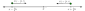
\includegraphics[width=.4\paperwidth]{deduction}
    \end{figure}

    \begin{definition}[Advection equation]
        \begin{equation*}
            u_{t}+du_{x}=0.
        \end{equation*}
    \end{definition}

    \begin{definition}[Diffusion equation]
        \begin{equation*}
            u_{t}=
            du_{xx}.
        \end{equation*}
    \end{definition}

    Let $h>0$, $h<<1$
\end{frame}

	\section{Heuristic derivation of Advection Differential Equation}

\begin{frame}
	\begin{definition}[Average concentration]
		Let $h>0$, $h\ll 1$.
		We define the \emph{average concentration}
		\begin{math}
			\averageconcentration
		\end{math}
		in a space-time cell
		\begin{math}
			\left[
				x-\frac{1}{2}h,
				+x\frac{1}{2}h
				\right]
			\times
			\left[
				0,T
				\right]
		\end{math}.

		\begin{equation*}
			\averageconcentration=
			\dfrac{1}{h}
			\int_{x-\frac{1}{2}h}^{x+\frac{1}{2}h}
			u
			\left(
			s,t
			\right)
			\dl s.
		\end{equation*}
	\end{definition}

	\begin{definition}[Mass flux]
		The mass flux is the product of
		\begin{equation*}
			J_{x}=
			c
			v_{x}.
		\end{equation*}

		\begin{itemize}
			\item

			      $J_{x}$ is the mass flux in $x$-direction.

			\item

			      $c$ is the concentration of the substance.

			\item

			      $v_{x}$ is the velocity of the substance in the
			      $x$-direction.
		\end{itemize}
	\end{definition}

	\begin{theorem}[Conservation law]
		If the species is carried along by a flowing medium with
		velocity
		\begin{math}
			a\left(x,t\right)
		\end{math},
		then the mass conservation law
		implies that the change of
		\begin{math}
			\averageconcentration
		\end{math}
		per
		unit of time is the net balance of inflow and outflow over
		the cell boundaries,
		\begin{equation*}
			\diffp{\averageconcentration}{t}=
			\dfrac{1}{h}
			\left[
				a
				\left(
				x-\frac{1}{2}h,t
				\right)
				u
				\left(
				x-\frac{1}{2}h,t
				\right)-
				a
				\left(
				x+\frac{1}{2}h,t
				\right)
				u
				\left(
				x+\frac{1}{2}h,t
				\right)
				\right].
		\end{equation*}
	\end{theorem}
\end{frame}

\begin{frame}
	\frametitle{Numerical Quadrature~(\citeauthor[p.~9]{Hundsdorfer2003})}

	\begin{definition}[Advection equation]
		\begin{equation*}
			\diffp{\concentration}{t}+
			\diffp{a\left(x,t\right)\concentration}{x}=
			0.
			% u_{t}+du_{x}=0.
		\end{equation*}
	\end{definition}

	\begin{definition}[Diffusion equation]
		\begin{equation*}
			\diffp{\concentration}{t}=
			\diffp{}{x}
			\left(
			d\left(x,t\right)\diffp{\concentration}{x}
			\right).
			% u_{t}=du_{xx}.
		\end{equation*}
	\end{definition}

	\begin{figure}[ht!]
		\centering
		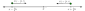
\includegraphics[width=.6\paperwidth]{deduction}
	\end{figure}
\end{frame}

\begin{frame}
	\begin{theorem}[Mass conservation law]
		If $\concentration$ is a concentration and
		\begin{equation*}
			M\left(t\right)\coloneqq
			\int_{0}^{1}
			u\left(x,t\right)
			\dl x
		\end{equation*}
		represents the mass in $\left[0,1\right]$ at time $t$, then
		$M$ is a conserved quantity.
	\end{theorem}

	\begin{proof}
		\begin{align*}
			\diff{M\left(t\right)}{t} & =
			\int_{0}^{1}
			u_{t}\left(x,t\right)
			\dl x=
			\int_{0}^{1}
			\left(
			-au_{x}\left(x,t\right)+
			du_{xx}\left(x,t\right)
			\right)\dl x                  \\
			                          & =
			-a\left(
			u\left(1,t\right)-
			u\left(0,t\right)
			\right)+
			d\left(
			u_{x}\left(1,t\right)-
			u_{x}\left(0,t\right)
			\right)=0.
		\end{align*}
	\end{proof}
\end{frame}

\section{The Advection Problem in One Dimension}

\begin{frame}
	\begin{definition}[space-time grid]
		Let $d\in\mathbb{N}$, $\Omega=\left(0,1\right)^{d}$, and $T>0$.
		For $K, N\in\mathbb{N}$, we set $\tau=\frac{T}{K}$ and
		$h=\frac{1}{N+1}$.
		We define the \emph{space-time grid domain}
		\begin{equation*}
			\overline{\mathcal{C}}^{\tau}_{h}=
			\overline{\Omega}_{h}\times
			{\left[0,T\right]}_{\tau}=
			\left\{
			\left(\mathbf{x},t_{k}\right)\mid
			\mathbf{x}\in\overline{\Omega}_{h},
			t_{k}=k\tau,
			k\in\left\{0,\dotsc,K\right\}
			\right\},
		\end{equation*}
		where we recall that
		\begin{math}
			\overline{\Omega}_{h}=
			\overline{\Omega}\cap
			\mathbb{Z}^{d}_{h}
		\end{math}.
		We define the \emph{discrete interior} of $\overline{C}^{\tau}_{h}$ to be
		\begin{equation*}
			\mathcal{C}^{\tau}_{h}=\Omega_{h}\times
			\left(0,T\right)_{\tau}.
		\end{equation*}
	\end{definition}

	\begin{definition}[space-time grid functions]
		Let $\mathcal{C}^{\tau}_{h}$ be a space-time grid domain.
		We denote by
		\begin{equation*}
			\mathcal{V}
			\left(
			\overline{\mathcal{C}}^{\tau}_{h}
			\right)=
			\left\{
			v\mid
			\overline{C}^{\tau}_{h}\to\mathbb{R}
			\right\}
		\end{equation*}
		be the space of \emph{space-time grid functions}.
		The spaces
		\begin{equation*}
			\mathcal{V}
			\left(
			\mathcal{C}^{\tau}_{h}
			\right),
			\mathcal{V}
			\left(
			\partial_{L}\mathcal{C}^{\tau}_{h}
			\right)
		\end{equation*}
	\end{definition}
\end{frame}

\begin{frame}
	\begin{definition}[space-time discrete norms]
		Let $d\in\left\{1,2\right\}$, $p\in\left[1,\infty\right]$, and
		$q\in\left[1,\infty\right)$.
		We define the \emph{space-time} norm
		\begin{equation*}
			\left\|
			v
			\right\|_{L^{q}_{\tau}\left(L^{p}_{h}\right)}=
				{\left(\tau
					\sum_{k=1}^{K}
					\left\|v^{k}\right\|^{q}_{L^{p}_{h}}
					\right)}^{\frac{1}{q}}
		\end{equation*}
		and
		\begin{equation*}
			\left\|
			v
			\right\|_{L^{\infty}_{\tau}\left(L^{p}_{h}\right)}=
			\max^{K}_{k=0}
			{\left\|
			v^{k}
			\right\|}_{L^{p}_{h}}
		\end{equation*}
	\end{definition}
\end{frame}

\begin{frame}
	\begin{definition}[Péclet number]
		Consider the simple constant-coefficient advection-diffusion
		equation
		\begin{equation*}
			u_{t}+
			au_{x}=
			du_{xx},\quad
			t>0,\quad
			0<x<L,
		\end{equation*}
		with the given initial profile $u\left(x,0\right)$.
		If $d>0$ we need boundary conditions at $x=0$ and $x=L$,
		such as Dirichlet conditions.
		On the other hand, for the pure advection problem we need
		only to prescribe the solution at the \emph{inflow} boundary,
		that is, at $x=0$ if $a>0$ and $x=L$ if $a<0$.
		If $d>0$ but $d\approx0$, or more precisely if the
		\emph{Péclet number}
		\begin{equation*}
			\left|a\right|\frac{L}{d}
		\end{equation*}
		is large, the Dirichlet condition at the outflow boundary
		will give rise to a \emph{boundary layer}.

		If the Péclet number $\left|a\frac{L}{d}\right|$ is large,
		the problem is called \emph{singularity perturbed}.
		% It is assumed that $d>0$, excluding the pure advection case.
		% where $L$ is the length of the spatial interval.
	\end{definition}
\end{frame}

	\input{section/advection}
	\input{section/diffusion}
}

\nocite{*}
\printbibliography

\end{document}
